\chapter{Einleitung}

% \begin{itemize}
%     \item Schüttgutsortierung ist ein wichtiges Thema \todo{hier vielleicht dieses 10\% der Energie Beispiel bringen?}
%     \item Anwendungsbereiche Schüttgutsortierung
%     \item Maschinelle Lernverfahren sind ein heißes Thema, dass bei vielen existierenden problemen Anwendung findet
% \end{itemize}

Schüttgüter und ihr Transport sind aus unserer modernen, globalisierten Welt nicht mehr wegzudenken.
% Ob es sich um Lebensmittel wie Getreide, Kaffeebohnen oder Zucker, Bergbauerzeugnisse wie Eisenerze oder Kohle, Granulate oder Pellets handelt, 
% ausschlaggebend für die Einstufung als Schüttgut ist, dass das Material lose in großen Mengen transportiert wird.
Als Schüttgüter werden solche Materialien bezeichnet, die lose in großen Mengen transportiert werden. 
Dazu gehören Lebensmittel wie Getreide, Kaffeebohnen oder Zucker, aber auch Bergbauerzeugnisse, wie zum Beispiel Erze oder Kohle. 
Auch Rohstoffe in Pellet-Form und Granulate zählen zu dieser Kategorie\,\cite[]{schulze2009}.
Laut dem Seefrachtbericht der Vereinten Nationen wurden im Jahr 2017 insgesamt 3196 Millionen Tonnen von den volumenmäßig wichtigsten Schüttgütern Eisenerze, Kohle und Getreide verschifft\,\cite[Unterabschnitt 1.A.2]{unitednationsconferenceontradeanddevelopment2018}.
Der Anteil, der für die Verarbeitung von Schüttgutmaterialien verwendeten Energie am globalen Energieverbrauch, wird mit 10 \% angegeben\,\cite[Abschnitt 1.2]{duran2012sands}.
In Zeiten der globalen Erwärmung ist der verantwortungsvolle Umgang mit Energie ein wichtiges Thema 
und eine effizientere Sortierung von Schüttgütern kann dazu beitragen.
Für das Sortieren solcher Schüttgüter gibt es verschiedene Methoden, 
wie zum Beispiel der Einsatz von Sieben, Magneten oder Flotationszellen.
Diese Sortiermethoden basieren auf unterschiedlichen physikalischen Eigenschaften der Schüttgutpartikel.
Im Rahmen dieser Arbeit wird die optische Schüttgutsortierung behandelt, 
die stattdessen anhand der optischen Eigenschaften der einzelnen Schüttgutpartikel sortiert.
% Eine Sortiermethode, die nicht auf die physikalischen Eigenschaften der Schüttgutpartikel aufbaut 
% sondern auf den Optischen, ist die bilddatenbasierte Schüttgutsortierung, um die es im Rahmen dieser Arbeit gehen soll.
% Ein Vorteil den diese Technik hat ist, dass sie besonders nicht-destruktiv ist, während beim mechanischen Sortieren die Gefahr besteht, dass einzelnen Partikel beschädigt werden könnten.
% In dieser Arbeit soll es insbesondere um eine nicht-destruktive Sortiervariante, nämlich die bilddatenbasierte beziehungsweise optische  gehen.
% Um die Qualität der Schüttgutsortierung zu steigern wird im Rahmen dieser Arbeit der Einsatz von neuronalen Netzen für die Bewegungsprädiktion der einzelnen Partikel erprobt.
In den letzten Jahren haben neuronale Netze für einige beeindruckende Fortschritte in verschiedenen Forschungsfeldern gesorgt,
wie zum Beispiel in den Bereichen der Bildverarbeitung und der Spracherkennung.
% In den letzten Jahren haben neuronale Netze für einige beeindruckende Fortschritte in verschiedenen Forschungsfeldern gesorgt 
% und ihre Stärken in der Mustererkennung sollen nun hier Einsatz finden.
Um die Qualität der Schüttgutsortierung zu steigern,
wird im Rahmen dieser Arbeit der Einsatz von neuronalen Netzen für die Bewegungsprädiktion der einzelnen Partikel erprobt.



% \todo{Einleitungstext}

\section{Motivation}

% \color{blue}
% \begin{itemize}
%     \item State of the Art: große Sortierer 
%     \item Kooperation ISAS IOSB, \textit{TrackSort} Projekt 
%     \item Flächenkamera
%     \item 2 geteiltes Problem: Tracking und Prediction
%     \item Fokus dieser Arbeit: Prediction
%     \item Bewegungsmodelle für verschiedene Schüttgüter von Hand finetunen ist viel Aufwand und schwer
%     \item Option: Neuronale Netze einsetzen! 
%     \item zwei verschiedene Problemstellungen:
%     \item 1. die Position des Teilchens im nächsten Zeitschritt. \textbf{NextStep} für Trackingphase
%     \item 2. die Position (und die Zeit) die das Teilchen beim Passieren des Düsenarrays haben wird. \textbf{Separator}
%     \item Aktuell: auf Messungen - kein Vollständiger Schätzer
% \end{itemize}
% \color{black}

% \todo[inline]{arbeit motivieren. Schüttgutsortierung ist ein interessantes Feld, das sich potenziell für ML anbietet.}
% \todo[inline]{auf jeden fall separator- und NextStep-Netze unterscheidung erwähnen}

Der Großteil der heute in der Industrie eingesetzten optischen Schüttgutsortierer verwendet Zeilenkameras.
Dabei muss die Annahme getroffen werden, dass die Schüttgutpartikel keinerlei Geschwindigkeit orthogonal zur Transportrichtung haben,
weil diese nicht erfasst werden kann.
In Abbildung~\ref{fig:predMissed} ist dargestellt wie es zu einer Fehlseparierung kommen kann, wenn diese Annahme verletzt wird. \\
Durch den Einsatz von Flächenkameras ist es möglich, die Position eines Partikels auf dem Förderband zu mehreren Zeitpunkten zu bestimmen.
Basierend auf diesen Informationen sollen die Trajektorien der einzelnen Partikel vorhergesagt werden.
Diese sollen dazu verwendet werden, die Sortierqualität zu steigern. 
Im Rahmen des \textit{TrackSort}-Projekts, 
einer Kooperation zwischen dem Lehrstuhl für Intelligente Sensor-Aktor-Systeme (ISAS) des Karlsruher Instituts für Technologie
und dem Fraunhofer-Institut für Optronik, Systemtechnik und Bildauswertung (IOSB), 
wurde die Verbesserung der Schüttgutsortierung durch den Einsatz von Trackingverfahren basierend auf den Daten von Flächenkameras betrachtet.
% \todo[inline]{passt das hier rein, oder soll ich das eher wo anders erwähnen?}

\begin{figure}[h]
    \centering
    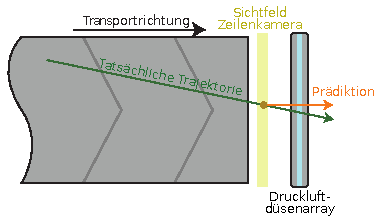
\includegraphics[width=0.8\textwidth]{PredictionMissed_translated_fixed.pdf}
    \caption[Darstellung einer Fehlseparierung basierend auf den Limitationen der Zeilenkamera. Übersetzt aus~~\cite{Pfaff2018}]
    {Darstellung einer Fehlseparierung durch die Annahme, dass es keine Bewegung orthogonal zur Transportrichtung gibt. 
    Übersetzt aus~\cite{Pfaff2018}.}
    \label{fig:predMissed}
\end{figure}


Um die zukünftigen Trajektorien der Partikel aus den vergangenen Positionen vorherzusagen, existieren verschiedene Bewegungsmodelle.
Diese liefern für unterschiedliche Situationen mit unterschiedlichen Bandgeschwindigkeiten, Schüttguttypen oder Prädiktionsdistanzen unterschiedlich gute Ergebnisse.  
Mittels neuronaler Netze können komplexe, nichtlineare Muster aus bestehenden Daten gelernt werden, ohne dass diese explizit angegeben werden müssen.
Es ist also denkbar, dass sie in der Lage sind, die Bewegungen des Schüttguts zu lernen.
Die für den Einsatz von neuronalen Netzen essenziellen Daten in ausreichender Menge zu sammeln, ist definitiv möglich. 
In dieser Arbeit soll nun erforscht werden, inwiefern der Einsatz von neuronalen Netzen zu einer Verbesserung gegenüber den bestehenden Ergebnissen führt.
Dabei wird exemplarisch mit Daten von dem \textit{TableSort}-Schüttgutsortierer gearbeitet.

Zu diesem Zweck sollen im Rahmen dieser Arbeit zwei verschiedene Prädiktionsprobleme durch neuronale Netze gelöst werden.
Einerseits soll vorhergesagt werden, an welcher Position sich ein Teilchen im nächsten Zeitschritt befinden wird.
Solche Netze werden von hier an als NextStep-Netze bezeichnet.
Die Visualisierung einer Probleminstanz mit dem dazugehörigen Label und einer von einem Netz generierten Prädiktion ist in Abbildung~\ref{fig:visualsNextstep} zu sehen.
Dies hilft dabei, das Zuordnungsproblem für Multi-Target-Tracking zu lösen.
Andererseits soll vorhergesagt werden, an welcher Position und wann ein Teilchen das Druckluftdüsenarray passieren wird.
Diese Problemstellung wird von sogenannten Separator-Netzen gelöst.
Die Visualisierung einer Probleminstanz mit dem dazugehörigen Label und einer von einem Netz generierten Prädiktion ist in Abbildung~\ref{fig:visualsSeparator} zu sehen.
Die Qualität dieser Prädiktion ist ausschlaggebend für den Erfolg der Separation.


\begin{figure}[p]
    \centering
    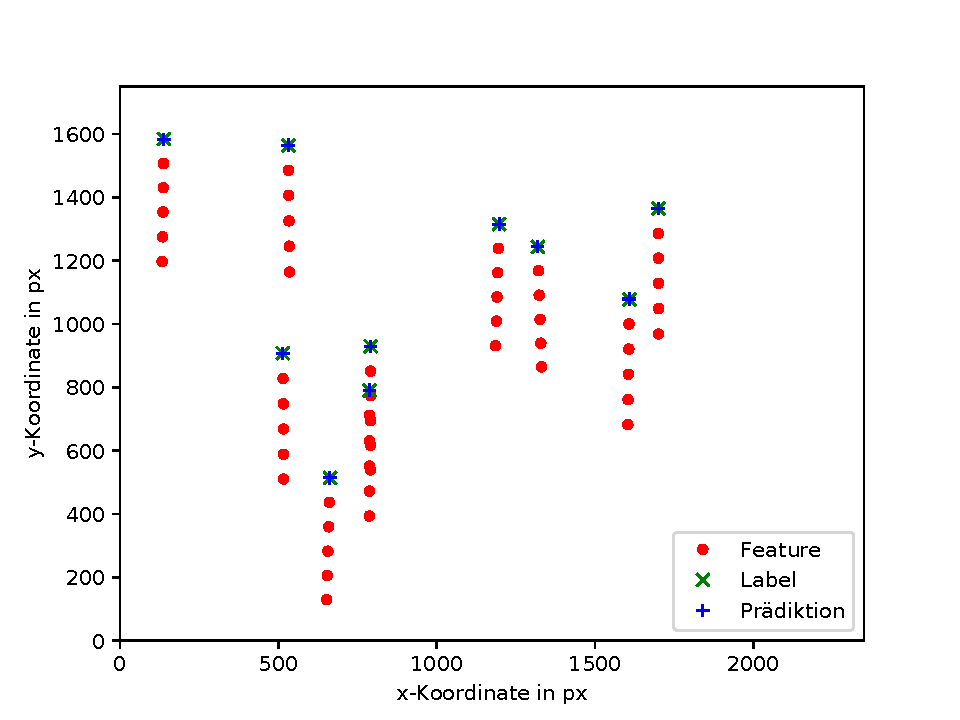
\includegraphics[width=0.725\textwidth]{NextStep-45kDecaySteps-ZylinderReal_2018-11-29_fixed.pdf}
    \caption[Visualisierung einer Probleminstanz eines NextStep-Netzes]{Visualisierung einer 
    Probleminstanz eines NextStep-Netzes. Die Transportrichtung ist entlang der \(\mathsf{y}\)-Achse.
    Die Features sind die zeitlich aufeinanderfolgenden, beobachteten Positionen eines Partikels.
    Die Prädiktion ist die Vorhersage des Netzes, wo das Partikel im nächsten Zeitschritt sein wird.
    Das Label ist die tatsächliche Position des entsprechenden Partikels im nächsten Zeitschritt.
    }
    \label{fig:visualsNextstep}
\end{figure}


\begin{figure}[p]
    \centering
    % \missingfigure{Real_Weizen_final_separatorExample.pdf}
	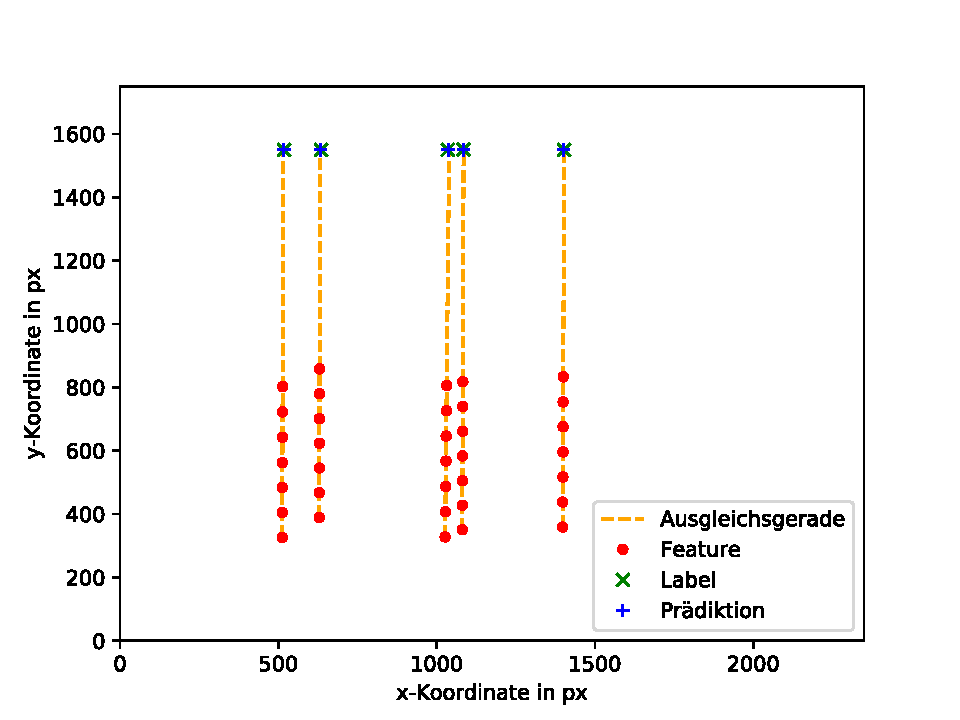
\includegraphics[width=0.725\textwidth]{Real_Weizen_final_separatorExample_fixed.pdf}
    \caption[Visualisierung einer Probleminstanz eines Separator-Netzes]{Visualisierung einer Probleminstanz 
    eines Separator-Netzes.
    Wie in Abbildung~\ref{fig:visualsNextstep} ist die Transportrichtung entlang der \(\mathsf{y}\)-Achse.
    Die Features sind erneut die beobachteten Positionen eines Partikels.
    % zeitlich aufeinanderfolgenden, --  entsprechende
    Die Prädiktion ist die vom Netz vorhergesagte Position, wo das Partikel das Druckluftdüsenarray passieren wird.
    Das Labels ist die tatsächliche Position, wo das Partikel das Druckluftdüsenarray passiert.
    Der Zeitpunkt, an dem das Druckluftdüsenarray passiert wird, ist nicht abgebildet.
    }
	
	\label{fig:visualsSeparator}
\end{figure}



\section{Aufbau der Arbeit}

% Das schreibe ich auf, wenn die Gliederung finalisiert ist.

% \begin{itemize}
%     \item Kapitel 2: Für das verständnis der Arbeit wichtige Grundlagen
%     \item Einerseits die von Neuronalen Netzen
%     \item Andererseits TableSort System und wie das was ich dann mit Neuronalen Netzen machen möchte bisher gemacht wird.
%     \item Kapitel 3: alles zu den Daten
%     \item Zuerst: selbst aufgenommene Daten. Was für Bilder wurden aufgenommen und wie wurden sie in den Zustand gebracht mit denen ich arbeiten will.
%     \item Dann: Die Simulierten Daten und der unterschied zu den aufgenommenen
%     \item Welche Form genau nehmen die Eingaben für mein Netz an und woher kommen die erwarteten Ausgaben.
%     \item Beschreibung der Vorgenommenen Datenaugmentierung
%     \item am Ende: eine kurze zusammenfassung wie viele Daten das jeweils sind.
%     \item Kapitel 4: Umsetzung und Implementierung
%     \item Benutzte Software
%     \item Beschreibung des Ablaufs mit dem ein Netz trainiert und evaluiert wird
%     \item Hyperparameter beschreiben und auf das Tuning eingegangen.
%     \item Kapitel 5: Evaluation
%     \item Hardware auf der Trainiert wurde
%     \item die mathematische Beschreibung der Modelle aus dem Stand der Technik für den Vergleich.
%     \item Evaluation der NextStep-Netze
%     \item Evaluation der Separator-Netze
%     \item Kapitel 6: Ganz zum Schluss - Fazit und Ausblick darauf was man noch so tun könnte in dem Feld
% \end{itemize}


Nachdem im ersten Kapitel eine kurze Einführung und Motivation für das Thema gegeben wurde, 
ist Kapitel~\ref{cap:basics} den theoretischen Grundlagen gewidmet, die für das Verständnis der restlichen Arbeit notwendig sind.
Dabei wird zu Beginn auf die Funktionsweise von neuronalen Netzen eingegangen, 
bevor die Funktionsweise und der Aufbau des \textit{TableSort}-Schüttgutsortierers beschrieben werden.
Am Ende des Grundlagenkapitels wird auf den aktuellen Stand der Technik eingegangen und erklärt, wie die Bewegungsprädiktion, 
die im Rahmen dieser Arbeit mittels neuronaler Netze durchgeführt werden wird, aktuell funktioniert.
% \todo{Verbessert ersetzen mit passenderer Formulierung}
Kapitel~\ref{cap:data} beschreibt die Daten, die dafür verwendet werden,
woher sie stammen, wie sie verarbeitet wurden und in welcher Form sie in die neuronalen Netze eingegeben werden.
Auch wird in diesem Kapitel auf die bereits existierenden Datensätze eingegangen, die mittels der \textit{Diskrete-Elemente-Methode} Schüttgut simuliert wurde,
und das verwendete Datenaugmentierungsverfahren beschrieben.
Danach wird auf den Umfang der verwendeten Daten eingegangen.
In Kapitel~\ref{cap:impl} wird die Implementierung der Arbeit thematisiert.
Dabei wird zunächst auf die verwendete Software eingegangen, bevor die Struktur des Codes beschrieben wird.
Es werden die für das Training und die Evaluation relevanten Hyperparameter beschrieben und die Optimierung derselben erläutert.
Kapitel~\ref{cap:Eval} beschäftigt sich mit der Evaluation der Ergebnisse.
% 
% Nachdem die Bewegungsmodelle erläutert werden, mit denen die Ergebnisse der neuronalen Netze verglichen werden,
% wird jeweils ein Blick auf den NextStep-Fall und den Separator-Fall geworfen und dann die Ergebnisse diskutiert.
Erst werden die verwendeten Bewegungsmodelle vorgestellt, die dann im NextStep-Fall und im Separator-Fall mit den Ergebnissen der neuronalen Netze verglichen werden.
Schließlich werden diese Ergebnisse diskutiert.
% 
Den Abschluss der Arbeit stellt Kapitel~\ref{cap:fazit} dar, in dem die Ergebnisse der Arbeit noch einmal zusammengefasst werden 
und ein Ausblick darauf gegeben wird, was in der Zukunft denkbare Fortführungen wären.
% \todo{aufbau Gliederung beschreiben. Ganz am Ende dann, wenn sich nichts mehr ändert}

